% ---------------------------------------------------------------------------
% The thermodiffusive lens in lean premixed hydrogen flames:
% measurements, derivations, and the analysis procedure.
%
% Build:  pdflatex ThermodiffusiveLens.tex   (twice, for the references)
% ---------------------------------------------------------------------------
\documentclass[11pt]{article}

\usepackage[margin=1in]{geometry}
\usepackage{amsmath,amssymb}
\usepackage{booktabs}
\usepackage{longtable}
\usepackage{graphicx}
\usepackage{tikz}
\usepackage{listings}
\usepackage[hidelinks]{hyperref}
\usepackage{xcolor}

\lstset{
  basicstyle=\ttfamily\small,
  breaklines=true,
  breakatwhitespace=false,
  columns=fullflexible,
  frame=single,
  framesep=4pt,
  rulecolor=\color{gray!50},
  backgroundcolor=\color{gray!5},
  showstringspaces=false,
}

\newcommand{\YH}{Y_{\mathrm{H_2}}}
\newcommand{\Le}{\mathrm{Le}}
\newcommand{\grad}{\nabla}
\newcommand{\dd}[2]{\frac{\mathrm{d}#1}{\mathrm{d}#2}}
\newcommand{\pd}[2]{\frac{\partial #1}{\partial #2}}

\title{The thermodiffusive lens in lean premixed hydrogen flames\\
       \large Measurements, derivations and the analysis procedure}
\author{Marc Day\\\small PeleAnalysis, branch \texttt{amr-complex}}
\date{\today}

\begin{document}
\maketitle

\begin{abstract}
Cellular structures in lean premixed hydrogen flames are characterised here
through the joint statistics of temperature and fuel mass fraction, taken in
range space rather than on any particular definition of a ``cell''. The
principal findings are: the lens structures visible between crossing $T$ and
$\YH$ contours are the \emph{hot-and-rich} quadrant of the $T$--$\YH$ plane,
and they capture fuel consumption to within $7\%$ of the best region of equal
volume that could be drawn; they are a level set of the excess-enthalpy scalar
$S = \theta + y - 1$, so a single threshold replaces the two; the Lewis number
measured from local flux ratios is $\Le = 0.313$; and at fixed temperature the
fuel mass fraction varies by a factor of $2.2$ with flame curvature, with
consumption following it. The curvature, lens and band-shape observations are
three views of one differential-diffusion imbalance. All numbers come from a
single plotfile of a four-level AMR simulation at one instant; the procedure
for reproducing and extending them is given in
Sections~\ref{sec:procedure}--\ref{sec:porting}.
\end{abstract}

\tableofcontents

% ===========================================================================
\section{What was measured, and on what}
\label{sec:case}

The data is a single plotfile, \texttt{plt29791}, from a lean premixed
hydrogen flame: a $1.86 \times 1.86 \times 3.72$~mm domain, periodic in $x$
and $y$, four AMR levels with a refinement ratio of 2, $373{,}043{,}200$ cells
in total, $35$ components, $98$~GB on disk. The base mesh is
$128\times128\times256$ with $\Delta x_0 = 14.53\,\mu$m. The unburnt
temperature is $T_u = 693$~K and the unburnt fuel mass fraction is
$Y_u = 1.325792\times10^{-2}$.

Two length scales govern what can be measured at which level. The thermal
thickness, defined as $\delta_T = \Delta T / \max|\grad T|$, is
$19.4\,\mu$m at level~1 and $16.5\,\mu$m at level~2, giving

\begin{center}
\begin{tabular}{lrrrr}
\toprule
level & 0 & 1 & 2 & 3 \\
\midrule
$\Delta x$ ($\mu$m) & 14.53 & 7.27 & 3.63 & 1.82 \\
cells per $\delta_T$ & 1.3 & 2.7 & 5.3 & 10.7 \\
\bottomrule
\end{tabular}
\end{center}

Quantities involving no derivatives --- the lens thresholds, the enrichment,
the explained variance --- are converged at level~1. Curvature is a second
derivative and is not: see Section~\ref{sec:curvature-resolution}.

% ===========================================================================
\section{Coarse-fine-aware gradients}
\label{sec:gradients}

Gradients are taken on the block-structured grid with the same treatment of
coarse-fine interfaces that the solver uses, not on a derived or dual
structure. A centred difference on a level's own ghost data is wrong at a
coarse-fine interface in a specific way: the ghost cell is an interpolation of
coarse data, so the stencil silently mixes two resolutions and the result is
neither the coarse nor the fine gradient. The error sits exactly on the
interface, which is a surface, so it does not converge away --- it only gets
thinner.

\texttt{Src/AMRGradient.cpp} instead builds a \emph{composite}
\texttt{MLPoisson} over the whole hierarchy, applies it, and takes the
face-centred fluxes the operator computes, averaging them to cell centres.
Two details are load-bearing:

\begin{itemize}
\item \texttt{mlmg.apply()} must precede \texttt{getFluxes}. The coarse-fine
      correction is established by the apply; \texttt{getFluxes} alone returns
      fluxes that have not seen it.
\item \texttt{MLPoisson}'s flux is $-\grad\phi$, not $\grad\phi$.
\end{itemize}

This follows \texttt{Src/grad.cpp}. Note that \texttt{Src/curvature.cpp}
builds its operators one level at a time inside a loop over levels, so its
curvature, normals and strain carry the interface artefact described above ---
while, ironically, its optional progress-variable smoothing is a composite
solve and therefore is coarse-fine aware.

\subsection{Verification}

\texttt{Tools/amrGradStatsTest.sh} runs 19 checks in each of 2D and 3D. The
exact tests use a linear field, for which MLMG's interface interpolation is
exact, so the only remaining error is floating point. Results are reported on
three regions separately --- all cells, interior cells, and the band within
two cells of a coarse-fine interface --- because a global norm cannot see a
surface defect.

The gate is $\mathrm{tol} = 64\,\varepsilon\,|\phi|_{\max}/\Delta x$, and
$/\Delta x^2$ for curvature, since a difference quotient divides by $\Delta
x$. With the refined patch at the low corner the result is bit-exact; at the
high corner the same code gives $7\times10^{-15}$, which is $32\varepsilon$
amplified by $1/\Delta x$ at $\Delta x = 1/128$.

Each test is paired with \texttt{per\_level=1}, which builds one single-level
operator per level --- what \texttt{curvature.cpp} does. It must fail, and
does, by a factor of $10^{14}$ relative to the tolerance, entirely within the
coarse-fine band. A gate nothing can fail is not a gate.

% ===========================================================================
\section{The lens}
\label{sec:lens}

\subsection{Orientation}

The lens is the region between crossing $T$ and $\YH$ contours. In range
space, $T$ and $\YH$ are anti-correlated, so the data occupies a band running
from (cold, rich) to (hot, lean). The quadrant $\{T > t_2\} \cap \{\YH <
t_1\}$ is therefore the \emph{burnt corner}: all products, no reaction. It
gives an enrichment of $0.3\times$, worse than random.

The lens is the off-band quadrant,
\begin{equation}
  L(t_1,t_2) = \{\, T > t_2 \,\} \cap \{\, \YH > t_1 \,\},
\end{equation}
gas that is simultaneously hotter \emph{and} richer than the main band
permits. This is the super-adiabatic crest.

\subsection{Monotonicity}

Writing $C(t_1,t_2)$ for the volume integral of the consumption density
$q = -\dot{\omega}_{\mathrm{H_2}}$ over $L$, tightening either threshold
shrinks the region. Measured on the 7641 occupied bins of the fine
$(T,\YH)$ table, $C$ is monotone in both arguments exactly, and \emph{no bin
has a negative conditional mean consumption density}, so the monotonicity is
guaranteed rather than merely observed. The nested family $C_b < C_a$ is
well posed.

\subsection{Efficiency against the best possible region}

A high $R^2$ for $q$ given $(T,\YH)$ says a good function $\psi(T,\YH)$
exists; it says nothing about whether $\psi$'s level sets are shaped like
quadrant corners. The sharp test is to compare the lens against the
\emph{optimal} region of the same volume, which is a superlevel set of $\psi$
and whose boundary is by definition a contour of consumption density.

\begin{center}
\begin{tabular}{rrrrrrrr}
\toprule
budget & optimal & lens & $\YH - Y_L(T)$ & lens/opt & $t_2$ (K) & $t_1$ & enrichment \\
\midrule
0.20\% & 11.57\% & 10.23\% & 10.22\% & 0.884 & 1481 & $2.52\times10^{-3}$ & $51.4\times$ \\
0.50\% & 25.68\% & 23.53\% & 22.54\% & 0.916 & 1469 & $1.83\times10^{-3}$ & $47.3\times$ \\
0.87\% & 40.11\% & 37.27\% & 35.01\% & \textbf{0.929} & 1446 & $1.35\times10^{-3}$ & $42.9\times$ \\
2.00\% & 69.32\% & 65.12\% & 60.69\% & 0.939 & 1268 & $8.63\times10^{-4}$ & $32.9\times$ \\
5.00\% & 94.09\% & 93.03\% & 86.55\% & 0.989 & \phantom{0}889 & $3.11\times10^{-4}$ & $18.8\times$ \\
\bottomrule
\end{tabular}
\end{center}

The lens captures $93\%$ of what the best possible region of identical volume
captures, rising to essentially $100\%$ at larger budgets. The pair of
contours is very nearly the right shape, not merely a convenient one.

\subsection{Optimality condition}

For $L(t_1,t_2)$, maximising $C$ at fixed volume $V$ requires $\grad C =
\lambda \grad V$. Since
\begin{equation}
  \pd{C}{t_2} \Big/ \pd{V}{t_2}
    = \frac{\int_{\YH>t_1} q \,\mathrm{d}A}{\int_{\YH>t_1} \mathrm{d}A}
    \Bigg|_{T=t_2}
  = \langle q \rangle_{T\text{-face}},
\end{equation}
and likewise for the other face, the condition reduces to
\begin{equation}
  \boxed{\;\langle q \rangle_{T\text{-face}}
       = \langle q \rangle_{Y\text{-face}} = \lambda\;}
\end{equation}
The optimal corner sits where \emph{both bounding faces lie on the same
consumption-density level}, and $\lambda$ is that level. This is the rigorous
form of the observation that the contour intersection follows the consumption
contours. Measured, the face-mean ratio is $1.00$--$1.12$ over the useful
range (median $1.07$ for $\dot{\omega}_{\mathrm{H_2}}$, $1.02$ for heat
release), departing only where $t_1$ reaches the lowest occupied bin.

\subsection{A one-parameter family}

There is no useful functional $t_1(t_2)$, because the optimum is nearly
degenerate in $t_2$: a single fixed $t_2 \approx 1398$~K retains $0.917$ of
the full two-parameter optimum across budgets from $0.2\%$ to $5\%$. A
constant offset above the band fails --- $t_1 - Y_L(t_2)$ scatters by $2.7$
times its mean.

The better one-parameter form thresholds the excess fuel above the band,
$\YH - Y_L(T)$, where $Y_L(T) = \langle \YH \mid T\rangle$. It matches the
two-threshold lens and beats it at tight budgets. Every \emph{linear}
selector fails outright: $T$ alone, $\YH$ alone, and the best rotated
combination all capture under $1.3\%$ of the consumption at the $0.87\%$
budget, because the band is strongly curved. The structure is intrinsically a
departure from the manifold, which is why a contour intersection works and no
blended progress variable would.

\subsection{What the angle of intersection does not add}

The transversality measure
$\sin\theta = |\grad a \times \grad b| / (|\grad a||\grad b|)$ vanishes
wherever $b$ is locally a function of $a$, for any monotone relation, and so
is a pointwise, threshold-free measure of where a single progress variable
fails. Adding it as a third coordinate raises $R^2$ for
$\dot{\omega}_{\mathrm{H_2}}$ from $0.867$ to $0.873$ --- against a null
control (\texttt{normalx\_temp}, which by the $x$-periodicity of the domain
should carry nothing) of $+0.0002$. The increment is real but negligible:
given the \emph{pair of values} $(T,\YH)$, the angle at which the contours
cross says nothing further about the local consumption rate. The lens is
characterised by which contours bound it, not by the geometry of the crossing.

% ===========================================================================
\section{The differential-diffusion postulate}
\label{sec:postulate}

\subsection{Statement}

With $\theta = (T-T_u)/(T_{ad}-T_u)$, $y = \YH/Y_u$ and $D = \alpha/\Le$,
subtracting the species and energy transport equations gives, for the
excess-enthalpy scalar $S = \theta + y - 1$ (zero in the unburnt gas and in
any $\Le=1$ planar flame),
\begin{equation}
  \pd{S}{t} + \mathbf{u}\cdot\grad S
    = \grad\!\cdot(\alpha \grad S)
    + \grad\!\cdot\!\big[\alpha(\tfrac{1}{\Le}-1)\grad y\big].
  \label{eq:S}
\end{equation}
The source is precisely the failure of the fuel diffusive flux and the
conductive heat flux to cancel. Splitting the Laplacian into normal and
surface parts, $\grad^2 y = \partial^2_n y + \kappa|\grad y|$, the curvature
contribution to the source is
\begin{equation}
  \alpha\left(\frac{1}{\Le}-1\right)\kappa\,|\grad y|.
  \label{eq:source}
\end{equation}

\paragraph{Postulate.} \emph{The lens is the set $S > 0$: the region where
differential diffusion has delivered more fuel than conduction has carried
heat away. Its boundary is a level set of $S$, which to leading order is
$\YH - Y_L(T)$, and it forms at flame elements convex toward the reactants.}

With $\Le = 0.313$ the coefficient $(1/\Le - 1) = 2.23$ is of order unity: the
effect is strong because hydrogen is this diffusive, not marginally so.

\subsection{Test and result}
\label{sec:postulate-test}

The prediction is specific: at fixed temperature, $\langle \YH \rangle$ must
rise as $\kappa$ becomes more negative. It holds at every temperature from
$740$ to $1878$~K without exception, across 47 bins. At $1246$~K,

\begin{center}
\begin{tabular}{lrr}
\toprule
curvature band & $\langle \YH \rangle$ & $\langle q \rangle$ ratio to cusps \\
\midrule
$\kappa < -3\times10^{4}$ (crest) & $5.47\times10^{-3}$ & --- \\
$-3\times10^{4}$ to $-1\times10^{4}$ & $5.00\times10^{-3}$ & \\
$-1\times10^{4}$ to $1\times10^{4}$ & $4.35\times10^{-3}$ & \\
$1\times10^{4}$ to $3\times10^{4}$ & $3.42\times10^{-3}$ & \\
$\kappa > 3\times10^{4}$ (cusp) & $2.46\times10^{-3}$ & $2.83$ \\
\bottomrule
\end{tabular}
\end{center}

A factor of $2.2$ in fuel mass fraction at identical temperature. Over the
$\pm10^{5}$ curvature range the induced spread is $5.6\times10^{-3}$,
comparable to $Y_L$ itself --- an order-unity effect, not a perturbation. The
consumption ratio between crests and cusps at fixed $T$ is $2.6$ through the
preheat zone, rising to $4$--$8$ through the reaction zone, so the chain
$\kappa \rightarrow$ enrichment $\rightarrow$ consumption is visible at fixed
temperature and is therefore not a consequence of crests merely being hotter.

\subsection{The gradient scaling: supported, with a gap}

If enrichment accumulates over a diffusive residence time $\tau \sim
\delta^2/\alpha$, then integrating \eqref{eq:source} gives
$\mathrm{d}\YH/\mathrm{d}\kappa \approx (1/\Le-1)\,|\grad \YH|\,\delta^2$, so
the ratio $(\mathrm{d}\YH/\mathrm{d}\kappa)/\langle|\grad \YH|\rangle$ should
be constant. Measured over $900$--$1600$~K it is $9.57\times10^{-11}$~m$^2$
with $31\%$ scatter, while $|\grad \YH|$ itself varies by a factor of $2.3$
--- the constancy is the non-trivial part and it holds.

The implied length, however, is $\delta = 6.6\,\mu$m against a measured
thermal thickness of $19.4\,\mu$m: a factor of $2.9$ in $\delta$, or $8.6$ in
$\delta^2$. This is an order-of-magnitude consistency check that passed, not a
quantitative confirmation. The residence-time step is dimensional analysis
with an unspecified constant, and the curvature is taken at level~1 where it
is least reliable. Resolving this needs either trajectory integration or a
level-3 repeat; see Section~\ref{sec:open}.

% ===========================================================================
\section{The Lewis number}
\label{sec:lewis}

\subsection{Two estimators from the same first integrals}

In the preheat zone, with constant mass flux $m = \rho u$, the species and
energy equations integrate once to
\begin{equation}
  \rho D \dd{\YH}{x} = m\,(\YH - Y_u), \qquad
  \lambda \dd{T}{x} = m\,c_p\,(T - T_u).
\end{equation}
Writing $\xi = Y_u - \YH$ and $\tau = T - T_u$ and dividing,
\begin{equation}
  \dd{\xi}{\tau} = \Le\,\frac{\xi}{\tau}
  \qquad\Longrightarrow\qquad
  \xi \propto \tau^{\Le}.
  \label{eq:powerlaw}
\end{equation}
So the curvature of the $T$--$\YH$ band \emph{is} a power law whose exponent
is the Lewis number, and $\Le<1$ is exactly what makes it concave. Two
estimators follow, identical in a 1-D flame:
\begin{align}
  \Le^{(A)} &= \dd{\ln \xi}{\ln \tau}
    &&\text{(band curvature)} \\
  \Le^{(B)} &= \frac{|\grad \YH|}{|\grad T|}\cdot\frac{\tau}{\xi}
    &&\text{(local flux ratio)}
\end{align}

\subsection{They disagree, and why}

\begin{center}
\begin{tabular}{lll}
\toprule
estimator & preheat value & status \\
\midrule
band curvature $\Le^{(A)}$ & $0.44$ & biased high by $45\%$ \\
flux ratio, $\xi$ from $\langle \YH|T\rangle$ & $0.30$ & partly contaminated \\
flux ratio, $\xi$ per bin & $\mathbf{0.313}$ & clean; IQR $0.281$--$0.342$ \\
literature, lean H$_2$--air & $\approx 0.3$ & independent \\
\bottomrule
\end{tabular}
\end{center}

The disagreement is not about $\Le$. It is the statement
\begin{equation}
  \dd{\langle \YH | T\rangle}{T} \;\neq\; \frac{\langle|\grad \YH|\rangle}{\langle|\grad T|\rangle}.
\end{equation}
At $T\approx770$~K the band slope is $2.19\times10^{-5}$ and the mean-gradient
ratio is $1.46\times10^{-5}$. The conditional mean $\langle \YH|T\rangle$ is
not a path through a flame; it is an average over flame elements at different
enrichment, so its slope is inflated by the very differential diffusion being
measured. \textbf{The band-curvature estimator must not be used for $\Le$.}
It is retained in the tooling only because the \emph{shape} it describes is
what the lens exploits.

\subsection{Apparent Lewis number as a diagnostic}

Restricted to $713$--$1000$~K and split by the sign of $S$:

\begin{center}
\begin{tabular}{lrr}
\toprule
region & volume & $\Le$ apparent \\
\midrule
$S > 0$ (rich side, the lens) & $1.060\%$ & $0.378$ \\
$S \le 0$ (lean side, the cusps) & $0.673\%$ & $0.279$ \\
\bottomrule
\end{tabular}
\end{center}

This is not a transport coefficient varying --- the mixture is the same.
$\Le^{(B)}$ equals the true Lewis number only where the first integrals hold,
and the postulate says they fail inside the lens by exactly the
differential-diffusion source. Smaller $\xi$ on the rich side inflates
$\tau/\xi$. The $35\%$ split therefore \emph{measures the imbalance} using
only $\grad \YH$, $\grad T$, $T$ and $\YH$, with no reference to reaction
rates, curvature or heat release. The true transport value lies between, near
$0.31$.

\subsection{Temperature dependence}

$\Le^{(B)}$ rises from $0.31$ at $723$~K to $0.43$ at $1374$~K. This is
\emph{not} the temperature dependence of the transport coefficients: for
H$_2$ in N$_2$, $D \propto T^{1.7}$ and $\alpha = \lambda/\rho c_p \propto
T^{1.7}/c_p$, so $\Le \propto 1/c_p$ should fall slightly. The observed rise
tracks heat release, as the no-reaction assumption behind the first integrals
fails.

% ===========================================================================
\section{Curvature and resolution}
\label{sec:curvature-resolution}

Curvature is computed as $\kappa = \grad\!\cdot\mathbf{n}$ with the normal
regularised as
\begin{equation}
  \mathbf{n} = \frac{\grad T}{\max\!\big(|\grad T|,\; f\big)},
  \qquad f = 10^{-2}\max|\grad T|,
\end{equation}
dividing by $\max(|\grad T|, f)$ rather than zeroing below a floor. Hard
zeroing makes the normal field jump from zero to unit length across the floor
contour, and the divergence of that jump is a spurious curvature sitting on a
level set of $|\grad T|$ --- an artefact that looks exactly like a flame
structure. The regularised form is continuous everywhere.

The floor governs $66.27\%$ of the volume but only $0.16\%$ of the
consumption, so it costs nothing.

\paragraph{The extremum is mesh noise at every level.}

\begin{center}
\begin{tabular}{lrrr}
\toprule
 & level 1 & level 2 & ratio \\
\midrule
$\Delta x$ & $7.27\,\mu$m & $3.63\,\mu$m & 0.50 \\
$\max|\grad T|$ & $7.78\times10^{7}$ & $9.12\times10^{7}$ & 1.17 \\
$\max|\kappa|$ & $3.96\times10^{5}$ & $7.78\times10^{5}$ & \textbf{1.96} \\
$\max|\kappa|\cdot\Delta x$ & \textbf{2.88} & \textbf{2.83} & --- \\
\bottomrule
\end{tabular}
\end{center}

Halving $\Delta x$ doubled $\max|\kappa|$. The first derivative is converging
(it grew by $1.17\times$, not $2\times$); the second derivative's extremum is
not, and will keep doubling. This is expected of any finite-difference second
derivative and means \textbf{the maximum is the wrong statistic}: use the
volume-weighted distribution, read where there is a flame. At level~2, $63\%$
of the flame volume has $|\kappa| < 3\times10^{4}$, a radius above $33\,\mu$m
or nine cells, which is adequately resolved.

\paragraph{On smoothing.} \texttt{curvature.cpp} offers a pre-smoothing step,
$(I - \beta\grad^2)\tilde\phi = \phi$, solved compositely. It would produce
finite, smooth, plausible curvatures --- which is the danger, since their
values would be set by $\beta$ rather than by the flame. At the default
\texttt{smoothing\_time}~$=10^{-7}$, $\sqrt{\beta} = 316\,\mu$m against a
$19.4\,\mu$m flame in a $1.86$~mm box: it would erase the cellular pattern.
Matching the flame scale needs $\beta \approx \delta_T^2 \approx
3.8\times10^{-10}$, some $250\times$ smaller. More fundamentally, the
high-$|\kappa|$ tail \emph{is} the thermodiffusive signature, so smoothing
attenuates exactly what is being measured. It is the right tool for the cell
envelope at a chosen scale; it is the wrong tool for recovering curvature the
mesh did not resolve. If used, sweep $\beta$ and report what is stable.

\paragraph{Sign convention.} \texttt{amrGradStats} uses $\mathbf{n}$ pointing
toward the \emph{products}; \texttt{curvature.cpp} and the combustion
literature point it toward the reactants. The two curvatures are therefore
negatives of one another. In this document $\kappa < 0$ is a crest, convex
toward the reactants. In the standard convention the central result reads:
positive curvature burns roughly ten times faster than negative.

% ===========================================================================
\section{Synthesis}
\label{sec:synthesis}

The three threads are one mechanism.

\begin{itemize}
\item The \textbf{band curvature} in the $T$--$\YH$ plane is the power law
      $\xi \propto \tau^{\Le}$, so $\Le = 0.313$ sets its shape.
\item The \textbf{lens} is a level set of $S = \theta + y - 1$, which is the
      accumulated differential-diffusion imbalance. This is why the
      one-parameter selector $\YH - Y_L(T)$ matches a two-threshold family,
      and why every linear selector fails.
\item The \textbf{curvature--consumption correlation} is the source of $S$,
      with coefficient $(1/\Le - 1) = 2.23$.
\end{itemize}

The $47\times$ consumption enrichment found by sweeping thresholds is that
mechanism seen through a quadrant approximation.

This also answers the question the effort began with. A cell is a connected
component of $\{S > s\}$: one threshold rather than two, monotone by
construction, and --- once $Y_L^0(T)$ comes from a 1-D flame rather than from
the field itself --- meaning the same thing in every snapshot, which is the
property needed to relate elements through time.

% ===========================================================================
\section{The tools}
\label{sec:tools}

Three libraries and seven programs, in four layers, each layer resting on the
one before. Line counts are given because the ratio is the point: the tests are
bigger than the things they test.

\subsection{Layer 1 --- a cell structure you can trust on an adaptive mesh}

The hard part of working with adaptive mesh data is not the physics, it is the
bookkeeping. A plotfile is a stack of nested grids at different resolutions.
Anything you measure --- a volume, a surface area, a gradient --- has to behave
sensibly where a fine grid meets a coarse one, and has to behave sensibly where
the domain wraps around on itself. Get that wrong and the error does not show
up as noise everywhere; it shows up as a thin skin of wrongness along every
interface, which is much harder to notice and does not go away when you refine.

\paragraph{\texttt{AMRComplex}} builds, once, a structure that gets this right,
so that everything downstream can stop worrying about it. Think of the cell
centres of the input as the corners of a 3D mesh, and the blocks between them
as the mesh's cells. Where a fine grid abuts a coarse one, the block spanning
the gap is squashed --- several fine corners collapse onto one coarse corner
--- but it is still a block, and it still has a volume. Those squashed blocks
are what seal the interface.

The one decision that makes this work is how a corner is named. A corner is
identified by \emph{which cell it is} --- its level and its integer index ---
and never by where it sits in space. Two blocks share a corner because they
refer to the same cell, not because two floating-point coordinates happened to
agree to within some tolerance. The consequences are worth spelling out,
because all three are load-bearing:

\begin{itemize}
\item The structure is sealed at coarse-fine interfaces \emph{by construction}.
      There is no welding step and no tolerance to tune.
\item Periodic wrapping comes for free. AMReX's ghost-cell exchange copies the
      corner's stored name, and cannot alter an integer index while copying it,
      so the ghost cell beyond the high face ends up literally holding the
      low-face corner. The wrap identifies itself.
\item When this rule has been broken, the code has broken with it --- twice,
      both times in deciding which grid box owns a block that straddles a
      periodic seam. Both times the symptom was a volume that did not add up.
\end{itemize}

That last point is why there is a self-check. \texttt{verify()} adds up the
volumes of every block and compares the total against the volume of the domain,
which is a number known exactly in advance. If the blocks tile the domain, the
two agree to the last bit; if anything is missing, duplicated, or folded over,
they do not. It also checks that every internal face is shared by exactly two
blocks, which is the statement that the structure has no holes. Two of the
checks need a lookup table over every face or every block on each processor ---
two billion entries on a production case --- so those are off unless asked for,
and the cheap version of the same test always runs.

\subsection{Layer 2 --- surfaces and connected regions}

\paragraph{\texttt{AMRContour}} draws an isosurface: the surface where some
field equals a chosen value. Two decisions:

\begin{enumerate}
\item Each block is first chopped into tetrahedra, and the surface is traced
      through the tetrahedra rather than through the blocks directly. A
      tetrahedron cut by a surface has only three possible outcomes, all
      unambiguous. A cube has famously ambiguous cases --- situations where the
      data alone does not say whether two corners of a face are connected
      through the face or around it --- and resolving them inconsistently
      between neighbouring cubes tears holes in the surface. Chopping into
      tetrahedra removes the question rather than answering it.
\item A point on the surface is named by \emph{which edge it lies on}, and that
      edge by the pair of corners at its ends. Two blocks sharing an edge
      therefore arrive at the same surface point automatically, at any
      refinement level and across a periodic wrap. No merging of nearby points,
      no tolerance, and none of the cracks and misplaced vertices that follow
      from getting such a merge slightly wrong.
\end{enumerate}

It reports the surface area, how many triangles and vertices there are, whether
the surface is closed (every edge used by exactly two triangles --- a count that
comes out at exactly zero for a closed surface, at any processor count),
whether the triangles are consistently oriented, and the volume the surface
encloses. In 2D the same statements hold with line segments instead of
triangles, which is why the closure test is literally the same code.

\paragraph{\texttt{AMRSegment}} finds connected regions: given a threshold, which
blobs does it pick out, and which cells belong to which blob. Two properties
matter more than speed.

\emph{Periodic domains need no special handling.} The regions are grown through
the complex's own neighbour relationships, and those already know about the
wrap and about coarse-fine interfaces. No domain face ever enters the
calculation, so where you happen to have placed the boundaries cannot change
the answer.

\emph{Region labels do not depend on how the work was divided.} A region is
named after the smallest cell index it contains --- a property of the region
itself, not of which processor happened to find it. Run the same case on 1
processor or 64 and the labels are identical. That is what makes two
segmentations comparable at all: across processor counts, across candidate
definitions, and across time, which is the one that matters for following a
structure as it evolves.

\paragraph{The programs.}
\begin{itemize}
\item \texttt{amrSweep} walks a threshold through a field's range and reports,
      at each value, how many separate regions it picks out, how their sizes
      are distributed, and how much surface there is. Run it on several
      candidate fields and the tables are directly comparable --- which is the
      point, because what a ``cell'' is, is exactly the thing not yet known.
      What one looks for is a plateau in the region count, or a gap in the size
      distribution. Either would be a scale that does not depend on the
      threshold, and so a defensible definition. A featureless continuum is
      also an answer, and a more interesting one.
\item \texttt{amrLabel} writes a segmentation as a plotfile: one integer per
      cell saying which region it belongs to, on exactly the input's own grids,
      so it can be loaded alongside the original fields and overlaid directly
      in a viewer. It can also write the isosurface with each triangle tagged by
      the region it bounds. Region numbers are compact and ordered by size
      (1 is the largest) rather than being the raw cell index, which runs to
      hundreds of millions and would not survive being stored as a
      single-precision number.
\item \texttt{amrComplexVerify} and \texttt{amrContourVerify} build and check.
\item \texttt{surfMEFtoDAT} converts an extracted surface between file formats.
\end{itemize}

\subsection{Layer 3 --- gradients}

\paragraph{\texttt{AMRGradient}} (87 lines) takes derivatives. The whole content
of it is Section~\ref{sec:gradients}: ask the linear-solver machinery for the
gradient over the entire grid hierarchy at once, rather than one level at a
time, so that coarse-fine interfaces are handled the way the flow solver itself
handles them. Figure~\ref{fig:cf} is the reason this matters and the reason the
test suite measures what it measures.

\begin{figure}[t]
\centering
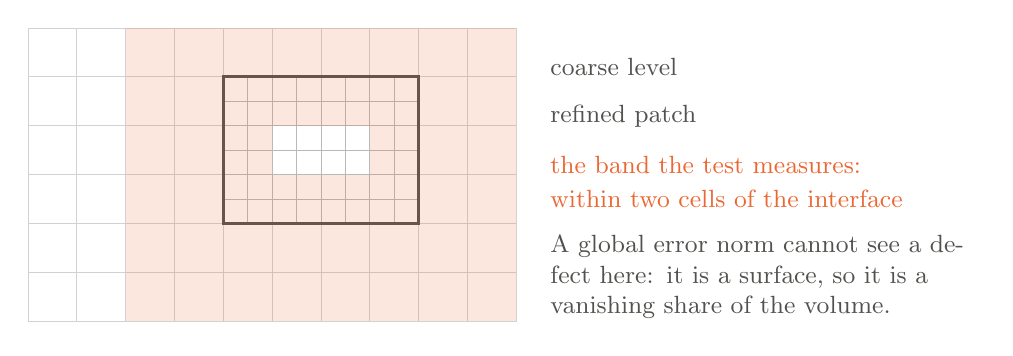
\begin{tikzpicture}[scale=0.62]
  \definecolor{band}{HTML}{EB6834}
  \definecolor{ink}{HTML}{52514E}
  \foreach \i in {0,...,9} \foreach \j in {0,...,5}
    \draw[gray!35,line width=0.3pt] (\i,\j) rectangle ++(1,1);
  \foreach \i in {8,...,15} \foreach \j in {4,...,9}
    \draw[gray!55,line width=0.25pt] (\i*0.5,\j*0.5) rectangle ++(0.5,0.5);
  \draw[ink,line width=1.1pt] (4,2) rectangle (8,5);
  \fill[band,opacity=0.16] (2,0) rectangle (4,6);
  \fill[band,opacity=0.16] (8,0) rectangle (10,6);
  \fill[band,opacity=0.16] (4,0) rectangle (8,2);
  \fill[band,opacity=0.16] (4,5) rectangle (8,6);
  \fill[band,opacity=0.16] (4,2) rectangle (8,3);
  \fill[band,opacity=0.16] (4,4) rectangle (8,5);
  \fill[band,opacity=0.16] (4,3) rectangle (5,4);
  \fill[band,opacity=0.16] (7,3) rectangle (8,4);
  \node[ink,anchor=west,font=\small] at (10.5,5.2) {coarse level};
  \node[ink,anchor=west,font=\small] at (10.5,4.2) {refined patch};
  \node[band,anchor=west,font=\small] at (10.5,3.2)
       {the band the test measures:};
  \node[band,anchor=west,font=\small] at (10.5,2.5)
       {within two cells of the interface};
  \node[ink,anchor=west,font=\small,text width=5.4cm] at (10.5,0.9)
       {A global error norm cannot see a defect here: it is a surface, so it is
        a vanishing share of the volume.};
\end{tikzpicture}
\caption{Why \texttt{amrGradVerify} reports three regions separately. A wrong
gradient at a coarse-fine interface lives on a two-dimensional surface inside a
three-dimensional volume, so it barely moves an error norm taken over
everything. Refining makes the skin thinner, not better.}
\label{fig:cf}
\end{figure}

\paragraph{\texttt{amrGradStats}} (357 lines) writes a new plotfile on the same
grids containing: the requested fields unchanged, their gradients and gradient
magnitudes, the angle between pairs of gradients, and optionally the direction
normal to a surface and that surface's mean curvature. Because the output is an
ordinary plotfile on the input's own grids, every downstream tool reads it with
no special handling.

\paragraph{\texttt{amrGradVerify}} (248 lines) measures the error against a case
whose answer is known exactly, and reports it on three regions separately: all
cells, interior cells, and the band shaded in Figure~\ref{fig:cf}. The split is
the entire tool.

\subsection{Layer 4 --- statistics in value space}

\paragraph{\texttt{AMRJointStats}} (254 lines) answers questions of the form
``if I know the temperature and the fuel fraction at a point, how much does
that tell me about the heat release there?'' It does this by sorting every cell
into a bin according to its field \emph{values} rather than its position, and
accumulating, per bin, the volume and the mean and spread of whatever responses
were asked for. From that it reports, for every combination of the chosen
variables, the fraction of the response's variation those variables account
for. Volumes are accumulated as integer cell counts times exact cell volumes,
so the total closes exactly rather than approximately, and the sums are
compensated so that the answer does not depend on how many processors ran it.

\paragraph{\texttt{amrJointFit}} (245 lines) is the program that drives it and
writes the table.

\subsection{Testing}

\begin{center}
\begin{tabular}{llr}
\toprule
suite & what it covers & lines \\
\midrule
\texttt{amrComplexMpiTest.sh}   & same answer at any processor count & --- \\
\texttt{amrComplexShapeTest.sh} & 13 grid layouts $\times$ 2 dimensions & 305 \\
\texttt{amrContourMefTest.sh}   & surface closure, parallel gathering & --- \\
\texttt{amrJointStatsTest.sh}   & volume closure, convergence, consistency & 385 \\
\texttt{amrGradStatsTest.sh}    & 19 checks per dimension & 369 \\
\texttt{amrBuildAndTest.sh}     & builds everything, runs all of the above & --- \\
\bottomrule
\end{tabular}
\end{center}

One rule runs through all of them: \textbf{every check is paired with a
deliberately broken version that it must catch.} Switches exist to reinstate
each defect that was ever found here --- the old ownership rule, the
too-narrow interface stitch, the one-level-at-a-time gradient, an inconsistent
subdivision --- and the suite fails if any of them passes. A check that cannot
be made to fail is not a check, and two of these caught a real regression while
merging two branches of this work.

\subsection{Analysis}

\paragraph{\texttt{lensAnalysis.py}} (506 lines) reads the tables
\texttt{amrJointFit} writes and nothing else, which is what lets any number in
this document be traced back to a file on disk. Five modes, one per question
asked in Sections~\ref{sec:lens}--\ref{sec:lewis}. \textbf{\texttt{runLensPipeline.sh}}
(204 lines) runs the whole chain in one command.

% ===========================================================================
\section{How the tools produce the result}
\label{sec:chain}

Three stages, each feeding the next.

\paragraph{Stage 1.} \texttt{amrGradStats} turns the raw plotfile into one
carrying $\nabla T$, $\nabla \YH$, their magnitudes, the angle between them,
and the curvature of the temperature field, with the heat release and the fuel
consumption rate carried through untouched.

\paragraph{Stage 2.} \texttt{amrJointFit} reduces that to four tables, each
asking a different question through its choice of binning variables:

\begin{center}
\begin{tabular}{llp{0.34\textwidth}}
\toprule
binned on & responses & question \\
\midrule
$(T, \YH)$ & heat release, $\dot\omega$ & where the consumption lives in the
  $T$--$\YH$ plane \\
\addlinespace[2pt]
$(T, \YH)$ & $|\nabla T|$, $|\nabla \YH|$ & the Lewis number, from the ratio of
  the two fluxes \\
\addlinespace[2pt]
$(T, \kappa)$ & $\YH$, $\dot\omega$ & how fuel and burning vary with curvature
  at fixed temperature \\
\addlinespace[2pt]
$(T, \YH, \kappa, |\nabla T|)$ & $\dot\omega$ & whether curvature adds anything
  the value pair does not already say \\
\bottomrule
\end{tabular}
\end{center}

\paragraph{Stage 3.} \texttt{lensAnalysis.py}, one mode per table.
Figures~\ref{fig:plane}--\ref{fig:curv} are its output.

\begin{figure}[p]
\centering
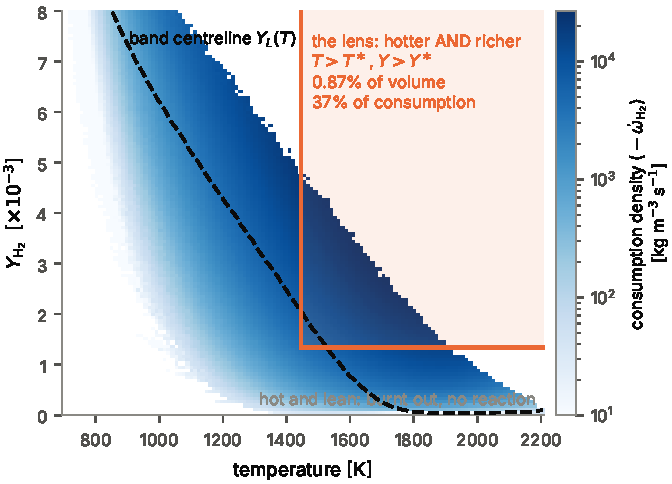
\includegraphics[width=0.92\textwidth]{figs/fig_plane.pdf}
\caption{Where the burning is, in value space. Every cell in the domain is
placed by its temperature and its fuel mass fraction, and shaded by how fast
fuel is being consumed there. The data occupies a curved band, because
temperature and fuel are strongly anti-correlated through a flame: the dashed
line is the band's centre. The lens is the orange quadrant --- gas that is
simultaneously \emph{hotter} and \emph{richer} than the band allows. It holds
0.87\% of the volume and 37\% of the consumption. The opposite corner, hot and
lean, is burnt-out product: no fuel left and nothing happening. This is why the
first orientation we tried, hot-and-lean, gave an enrichment \emph{below}
random.}
\label{fig:plane}
\end{figure}

\begin{figure}[p]
\centering
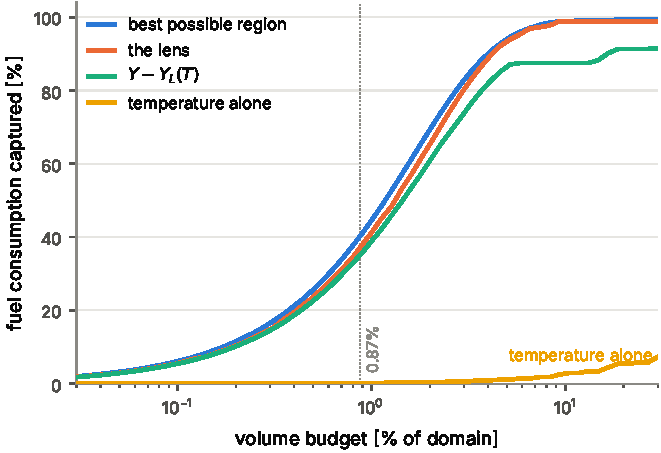
\includegraphics[width=0.86\textwidth]{figs/fig_capture.pdf}
\caption{How good the lens is, against the best that any region of the same
size could do. The upper curve is the theoretical optimum --- take the cells
with the highest consumption first, regardless of what shape that makes. At the
0.87\% operating point the lens captures 93\% of that, so a pair of contours is
very nearly the right shape and not merely a convenient one. Thresholding the
single quantity $Y - Y_L(T)$ does about as well with one parameter instead of
two. Temperature alone captures almost nothing, and neither does any straight
line drawn in the plane of Figure~\ref{fig:plane}: the structure is a departure
from the curved band, which no single blended progress variable can express.}
\label{fig:capture}
\end{figure}

\begin{figure}[p]
\centering
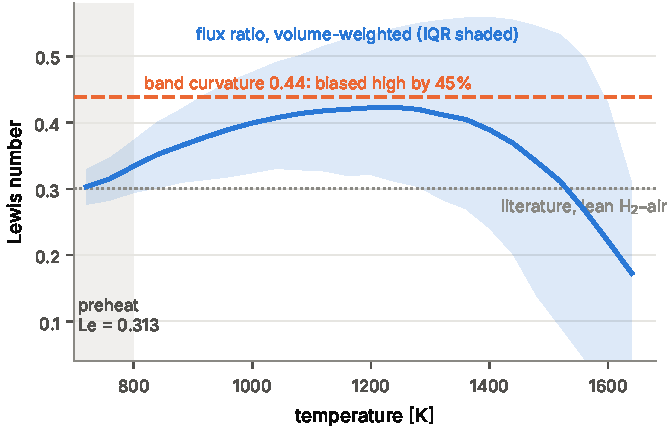
\includegraphics[width=0.86\textwidth]{figs/fig_lewis.pdf}
\caption{The Lewis number --- how fast hydrogen diffuses relative to heat ---
measured two ways from the same data. The solid curve is the ratio of the two
fluxes, measured locally. In the preheat zone, where the derivation behind it
is valid, it gives 0.313, matching the accepted value for lean hydrogen--air.
The dashed line is what the shape of the band in Figure~\ref{fig:plane} implies;
the two are identical in a one-dimensional flame, and they disagree here by
45\% because the band's centre is an average over flame elements at different
enrichment, and so is bent by the very effect being measured. The rise above
800~K is not transport: it is heat release invalidating the derivation.}
\label{fig:lewis}
\end{figure}

\begin{figure}[p]
\centering
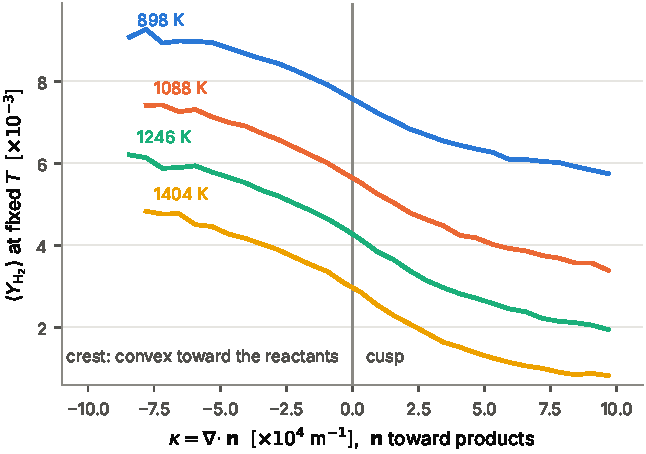
\includegraphics[width=0.86\textwidth]{figs/fig_curv.pdf}
\caption{The mechanism, in one picture. At \emph{fixed} temperature, there is
over twice as much fuel where the flame bulges toward the fresh gas as where it
is cupped the other way, and this holds at every temperature across the flame.
Since the temperature is the same along each curve, this cannot be explained by
the crests simply being hotter. It is hydrogen out-diffusing the heat that
would otherwise balance it --- and the consumption rate follows the same
ordering, by a factor of 2.6 in the preheat zone rising to 8 in the reaction
zone. Sign convention: the normal points toward the products, so negative
curvature is the crest; the combustion literature uses the opposite sign.}
\label{fig:curv}
\end{figure}

\paragraph{What the first two layers contribute, and what they do not.} The
lens result above uses neither \texttt{AMRContour} nor \texttt{AMRSegment}. It
is entirely an argument in value space, which is precisely what makes it
independent of any particular definition of a cell --- there are no blobs in it
and no threshold on anything spatial. Those tools answer the complementary
question: \texttt{amrSweep} asks whether a threshold-independent scale exists at
all, and \texttt{amrLabel} turns a chosen threshold into labelled regions that
load alongside the original data. The two halves meet at the end of
Section~\ref{sec:synthesis}. Once a cell is defined as a connected region of
$\{S > s\}$, with $S$ the excess-enthalpy scalar the value-space work
identified, it is \texttt{AMRSegment} that finds those regions and
\texttt{amrLabel} that writes them out --- and \texttt{AMRSegment}'s
processor-independent labelling is what would let the same region be
recognised in the next snapshot.

% ===========================================================================
\section{Procedure}
\label{sec:procedure}

\subsection{Build}

\begin{lstlisting}[language=bash]
cd $PELE_ANALYSIS/Src
for t in amrComplexVerify amrContourVerify amrSweep amrJointFit \
         makeTestPlt surfMEFtoDAT amrGradStats amrGradVerify ; do
    make -f GNUmakefile.AMRComplex AMREX_HOME=$AMREX_HOME \
         USE_MPI=TRUE COMP=gnu DIM=3 EBASE=$t -j16
done
\end{lstlisting}

\texttt{amrGradStats} and \texttt{amrGradVerify} are the only targets that
pull in \texttt{Boundary}, \texttt{AmrCore} and \texttt{LinearSolvers}; the
makefile adds those directories only for them. The first such build spends
several minutes compiling AMReX.

\paragraph{A recurring failure.} A driver must not be the case-variant of a
library source. On a case-insensitive filesystem \texttt{amrComplex.cpp}
\emph{is} \texttt{AMRComplex.cpp}: the second file written replaces the first,
one object is built instead of two, and the link fails on every library symbol
with ``referenced from \_main''. This has happened twice in this tree. Hence
\texttt{amrComplexVerify.cpp} and \texttt{amrJointFit.cpp}, and hence the name
guard in \texttt{Tools/amrBuildAndTest.sh}, which checks before anything is
compiled. A comment is not a check.

\subsection{Verify}

\begin{lstlisting}[language=bash]
cd $PELE_ANALYSIS
Tools/amrBuildAndTest.sh
DIM=3 Tools/amrGradStatsTest.sh
DIM=2 Tools/amrGradStatsTest.sh
\end{lstlisting}

Expect 19 passes in each dimension from the gradient suite. Do not proceed on
a failure: each check is paired with a control that must fail, so a suite that
passes vacuously would be silent.

\subsection{Run}

\begin{lstlisting}[language=bash]
Tools/runLensPipeline.sh --infile /path/to/plt29791 --case lean-h2 \
    --tu 693 --yu 1.325792e-2 --finest 1 --isper "1 1 0" --nproc 16
\end{lstlisting}

$T_u$ and $Y_u$ are case properties and must be the prescribed inflow values
--- the Lewis estimates are very sensitive to them ($\Le^{(A)}$ moves from
$0.44$ to $0.81$ if $T_u$ is taken as $680$ rather than $693$~K).

The pipeline writes, into \texttt{lens\_<case>\_L<n>/}: the derived plotfile;
four \texttt{amrJointFit} tables; and the analysis text files
\texttt{frontier.txt}, \texttt{band.txt}, \texttt{lewis.txt},
\texttt{postulate.txt} and \texttt{r2\_gated.txt}. Stages may be run
separately with \texttt{--stage grad|stats|analyse}.

\subsection{Analyse an existing table}

\begin{lstlisting}[language=bash]
Tools/lensAnalysis.py frontier  ty_fine.dat  --resp "I_R(H2)"
Tools/lensAnalysis.py lewis     lewis2d.dat  --Tu 693 --Yu 1.325792e-2
Tools/lensAnalysis.py postulate postulate.dat
Tools/lensAnalysis.py r2        ty_curv_gated.dat
\end{lstlisting}

\begin{sloppypar}
Columns are read from the header line rather than by position, so each mode
works on any \texttt{amrJointFit} table that carries the variables it needs.
\end{sloppypar}

% ===========================================================================
\section{Porting to a larger machine}
\label{sec:porting}

\subsection{Resources}

Derived from the $373$M-cell case: approximately $2.8$~GB of output per
component at full depth, and peak resident memory of about 20
component-equivalents (the state array plus per-variable scratch, face
MultiFabs and the Laplacian).

\begin{center}
\begin{tabular}{lrrr}
\toprule
\texttt{finestLevel} & cells & stage-1 output & stage-1 peak RSS \\
\midrule
1 & \phantom{0}25\,M & $\sim$4\,GB & $\sim$6\,GB \\
2 & 121\,M & $\sim$17\,GB & $\sim$30\,GB \\
3 & 373\,M & $\sim$53\,GB & $\sim$95\,GB \\
\bottomrule
\end{tabular}
\end{center}

Component count is the lever: dropping a variable from \texttt{vars} to
\texttt{carry} removes its gradient, magnitude and all its alignment pairs.

\subsection{GPU status, honestly}

\begin{center}
\begin{tabular}{llp{0.52\textwidth}}
\toprule
component & state & note \\
\midrule
\texttt{AMRGradient} & GPU-ready & MLMG apply, \texttt{getFluxes} and
  \texttt{average\_face\_to\_cellcenter} are all device-resident \\
\addlinespace[2pt]
\texttt{amrGradStats} & GPU-ready & pointwise work is \texttt{ParallelFor};
  one host loop remains, see below \\
\addlinespace[2pt]
\texttt{AMRJointStats} & host only & \texttt{forEachNode} with a host lambda
  and Kahan compensation into a host array \\
\addlinespace[2pt]
\texttt{AMRComplex} & host only & nine host loops in the traversal \\
\bottomrule
\end{tabular}
\end{center}

This split is fortunate: the expensive step at scale is the composite MLMG
apply, which is the GPU-capable part.

\paragraph{Known blocker.} The normal-floor volume diagnostic in
\texttt{amrGradStats.cpp} uses \texttt{AMREX\_LOOP\_3D}, a host loop, over
data that under a CUDA or HIP build lives in device memory. It is a
reduction and should become a \texttt{ReduceSum}. It has not been converted,
because it has not been possible to test a GPU build here. \textbf{Before
trusting any GPU result, build with \texttt{USE\_CUDA=TRUE} and run
\texttt{Tools/amrGradStatsTest.sh}}; if that diagnostic faults or reports a
nonsensical volume fraction, this is why, and the remedy is either the
\texttt{ReduceSum} conversion or guarding the diagnostic out under
\texttt{AMREX\_USE\_GPU}.

\paragraph{GPU build.}
\begin{lstlisting}[language=bash]
make -f GNUmakefile.AMRComplex AMREX_HOME=$AMREX_HOME \
     USE_MPI=TRUE USE_CUDA=TRUE COMP=gnu DIM=3 EBASE=amrGradStats -j16
\end{lstlisting}
One rank per GPU. The histogram stage of \texttt{AMRJointStats} would port as
a \texttt{ParallelFor} plus \texttt{Gpu::Atomic::Add} into a table of order
1~MB, but that work has not been done.

\subsection{Transfer checklist}

\begin{enumerate}
\item Clone AMReX at a known commit; this work was developed against
      \texttt{65db2e4e6}.
\item Clone PeleAnalysis, branch \texttt{amr-complex}.
\item Build the eight targets listed above; confirm the name guard passes.
\item Run \texttt{Tools/amrBuildAndTest.sh} and both dimensions of
      \texttt{Tools/amrGradStatsTest.sh}. All must pass before any science.
\item Copy or regenerate the plotfile. Record $T_u$ and $Y_u$ from the inputs
      file, not from the data.
\item Run the pipeline at \texttt{--finest 1} first. Compare
      \texttt{frontier.txt} and \texttt{lewis.txt} against
      Sections~\ref{sec:lens} and \ref{sec:lewis}. They should agree to the
      digits quoted.
\item Only then go to \texttt{--finest 3}.
\end{enumerate}

% ===========================================================================
\section{Open items}
\label{sec:open}

\begin{enumerate}
\item \textbf{$Y_L^0(T)$ from a 1-D laminar flame.} This is the weakest link.
      $Y_L(T)$ currently comes from the field under analysis, so it defines
      $S$, sets the lens threshold, and biased $\Le^{(A)}$ by $45\%$ --- all
      while containing the signal being measured. A Cantera or 1-D PeleLMeX
      solution at the case conditions removes the self-reference, makes the
      lens threshold portable across snapshots, and gives $\Le(T)$ from
      transport data as a fourth independent check on $0.313$.
\item \textbf{Curvature at level 3.} Everything in
      Section~\ref{sec:postulate} uses level~1, where $\max|\kappa| =
      2.85/\Delta x$. Noise degrades a correlation rather than creating one,
      so the monotone trend is safe, but the slope
      $-2.98\times10^{-8}$ --- and hence the $6.6\,\mu$m that should have been
      $19.4\,\mu$m --- will move with resolution.
\item \textbf{Residence time.} The $\delta^2$ in
      Section~\ref{sec:postulate} is dimensional analysis. Integrating
      \eqref{eq:source} along trajectories would turn an order-of-magnitude
      check into a quantitative one.
\item \textbf{Time sequence.} Everything here is one snapshot. The purpose of
      a reference-free, single-threshold cell definition is to track elements
      between snapshots; that has not been attempted.
\item \textbf{GPU.} See Section~\ref{sec:porting}.
\end{enumerate}

\end{document}
